\section{Canopy information and soybean yield}\label{sec:application}

\subsection{Repeated field trials with genomic adjustment}

Canopy development provides an observable phenotype before grain harvest.
The SoyNAM experiment recorded field imagery, grain yield and genome-wide
markers for recombinant inbred soybean lines \cite{xavier2017canopy}.
We ask whether average canopy coverage carries yield information after
genomic adjustment, and whether its association changes across the yield
distribution and between growing seasons. These questions distinguish
the information in an observed crop phenotype from the information
already available in its genotype.

The analysis uses the released \texttt{NAM::met} panel. Its 2013 and 2014
trials retain \SoyLines{} lines from \SoyFamilies{} families, with one
observed plot per line in each year, giving \SoyRecords{} records.
Each line forms a cluster of size two. The response is grain yield in
bushels per acre (bu/ac). Fitting expresses yield in units of ten bu/ac;
reported coefficients and prediction losses are transformed back to bu/ac.
Average canopy coverage is recorded as a
percentage and enters the model in units of ten percentage points.
The recorded yield means are \SoyYieldMeanThirteen{} and
\SoyYieldMeanFourteen{} bu/ac in 2013 and 2014, respectively.

Of the released \SoyOriginalMarkers{} marker columns, five are exact
duplicates. Their removal leaves \SoyMarkers{} distinct columns with
the same genomic linear span. Each marker has a separate coefficient
in each year. Together with the two year-specific canopy coordinates,
family contrasts, eight field-block indicators, year-specific maturity
splines and a check-plot spatial covariate, the full design contains
\SoyDimension{} columns. The genomic block enters all outcome and
adjustment searches. Family and the other prespecified adjustment
variables are retained in every selected model.

The spatial covariate is estimated from \SoyCheckPlots{} separate
check plots. A smooth field surface adjusts for row and column position
within each block, with check-strain and year effects included in its
calibration model. The analysed lines' yields do not enter that fit.
The profile criterion uses a line intercept with fixed $\Lambda=1$
on the stated working response scale.
We estimate the two canopy coordinates at $\tau=0.25,0.50,0.75$ using
$h=n^{-3/10}$. Complete lines exchange the selection and estimation
roles, with random ordering within families.

\subsection{Canopy associations across years and quantiles}

Figure~\ref{fig:soy-results} displays the canopy coordinates and their
simultaneous intervals. An increase of ten percentage points in
coverage corresponds to a positive profile association at all six
year--quantile combinations. At the median, the estimates are
\SoyMedianThirteen{} bu/ac in 2013 and \SoyMedianFourteen{} bu/ac in
2014, with intervals \SoyMedianThirteenInterval{} and
\SoyMedianFourteenInterval{}. These associations remain after adjusting
for the full genomic design, recorded maturity and field conditions.

The upper-quartile association is larger in 2014 by
\SoyUpperYearDifference{} bu/ac, with simultaneous interval
\SoyUpperYearDifferenceInterval{}. The corresponding lower-quartile
difference is \SoyLowerYearDifference{}, with interval
\SoyLowerYearDifferenceInterval{}. Within each year, the upper-minus-lower
contrasts have intervals containing zero. Thus the resolved contrast
concerns the upper-quartile association across years; the data leave
the within-year quantile differences less precisely determined.
The intervals allocate 5\% across the six coefficients and all five
prespecified contrasts, using the covariance of their common line
influence values.

\begin{figure}[t]
\centering
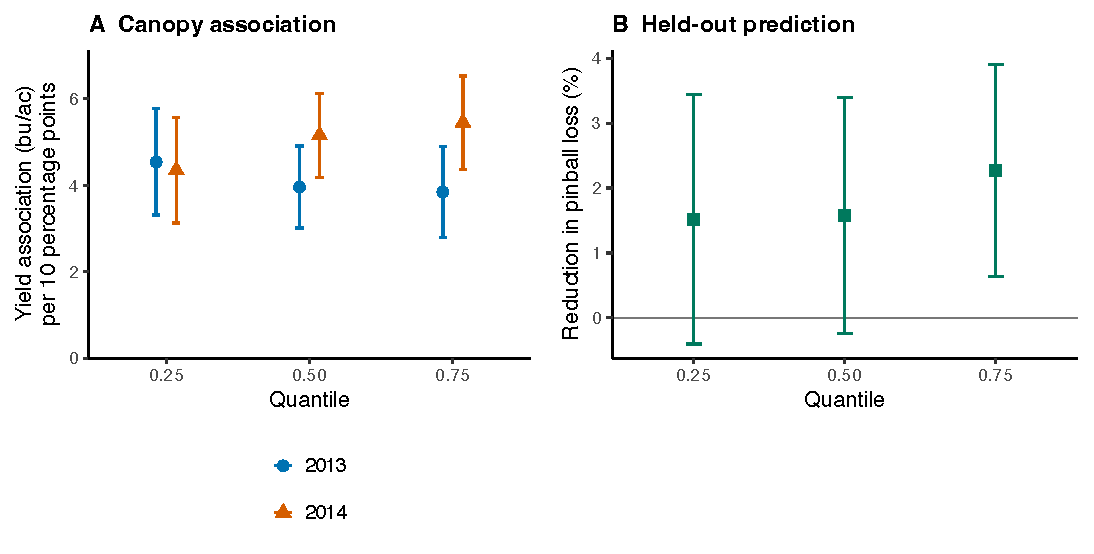
\includegraphics[width=\textwidth]{generated/soynam_profile/results.pdf}
\caption{Canopy information in the soybean trials. Panel A gives the year-specific profile coefficients per ten percentage points of coverage, with 95\% Bonferroni simultaneous intervals for the eleven prespecified coordinate and contrast parameters. Panel B gives the percentage reduction in held-out pinball loss when canopy is added to the joint predictor using genomic and field information. Its intervals use paired complete-line losses and the registered six-comparison Bonferroni adjustment. The prediction comparison uses training-only intercept calibration.}
\label{fig:soy-results}
\end{figure}


\subsection{Prediction for held-out lines}

A fixed set of \SoyTestLines{} lines supplies a separate prediction
evaluation. Their measurements from both years are withheld from
training. The remaining \SoyTrainingLines{} lines select model sizes
or penalties in three internal groups. All methods use the same
genomic and field information. The joint profile predictor is fitted
with and without the canopy variables; pooled quantile Lasso provides
an additional comparator with canopy information. Its complete convex
objective is solved with primal--dual certification. The prediction setting supplies the completed
check-plot calibration to every method. At the line level, the available
measurements are genotype and canopy; recorded maturity is excluded.
Year-specific intercept calibration uses internal validation residuals only.

\begin{table}[t]
\centering
\small
\caption{Mean pinball loss on the same held-out lines, in bu/ac. Each line receives equal weight across its two observations. Every predictor uses calibration estimated from training validation residuals.}
\label{tab:soy-prediction}
\begin{tabular}{rrr}
\toprule
$\tau$ & Joint with canopy & Joint without canopy \\
\midrule
0.25 & 2.670 & 2.711 \\
0.50 & 3.240 & 3.292 \\
0.75 & 2.545 & 2.604 \\
\bottomrule
\end{tabular}
\end{table}


Adding canopy information reduces upper-quartile prediction loss by
\SoyGenomicUpperGain{}\%, with simultaneous interval
\SoyGenomicUpperGainInterval{}\%. At the median, the estimated
reduction is \SoyGenomicMedianGain{}\%, with interval
\SoyGenomicMedianGainInterval{}\%; the lower-quartile reduction is
\SoyGenomicLowerGain{}\%, with interval
\SoyGenomicLowerGainInterval{}\%. The resolved upper-quartile gain
quantifies prediction information in the canopy measurements beyond
the genomic and field variables available to both models.


\subsection{Sensitivity and computation}

The seven registered settings yield \SoyFits{} completed fits.
Changing the bandwidth by factors of $0.75$ and $1.25$ changes a canopy
coefficient by at most \SoyBandwidthChange{} bu/ac. Separate settings
use $\Lambda=0.5$ and $2$, exclude the two lines with recorded maturity
above 180 days, and add block-specific quadratic spatial terms.
The upper-quartile year contrast ranges from \SoyYearContrastMinimum{}
to \SoyYearContrastMaximum{} bu/ac, with a positive simultaneous
interval in every setting. With the additional spatial terms, the
contrast is \SoySpatialYearContrast{}, with interval
\SoySpatialYearContrastInterval{}.
Supporting Information reports every interval and the numerical
diagnostics for these settings.

Selected model dimensions range from \SoyMinSelected{} to
\SoyMaxSelected{}. The paired-observation structure permits direct
elimination of line intercepts in the unsmoothed convex search,
followed by a reusable factorisation in the selected dimension.
Each solution retains its primal--dual certificate. The three
reference fits take \SoyReferenceMinMinutes{}--\SoyReferenceMaxMinutes{}
minutes each on an Apple M3 Max computer with 36 GB memory, including variable selection and
both bandwidth fits. Their influence values and original-coordinate
gradients are retained with the results.

Inference treats lines as independent conditional on the genomic,
family and field adjustment. The two growing seasons define the
observed trial conditions, and the fitted associations describe the
specified complete profile target in this population of lines.
